\section{Etat de l 'art}
   Cette partie concerne plus l architecture global des clouds. Leurs évolutions 
   au cours du temps ce qui mettra le point sur le besoin de la création d un nouveau 
   point d entrée.   

    \subsection{Le premier Cloud de MDI}
        \gls{CC} est le premier cloud fait maison de \gls{mdi} qui englobe un ensemble 
        de services pour les clients... L'architecture globale de ce cloud est comme le montre 
        le shema suivant: 

        \begin{figure}[ht]
            \centering
            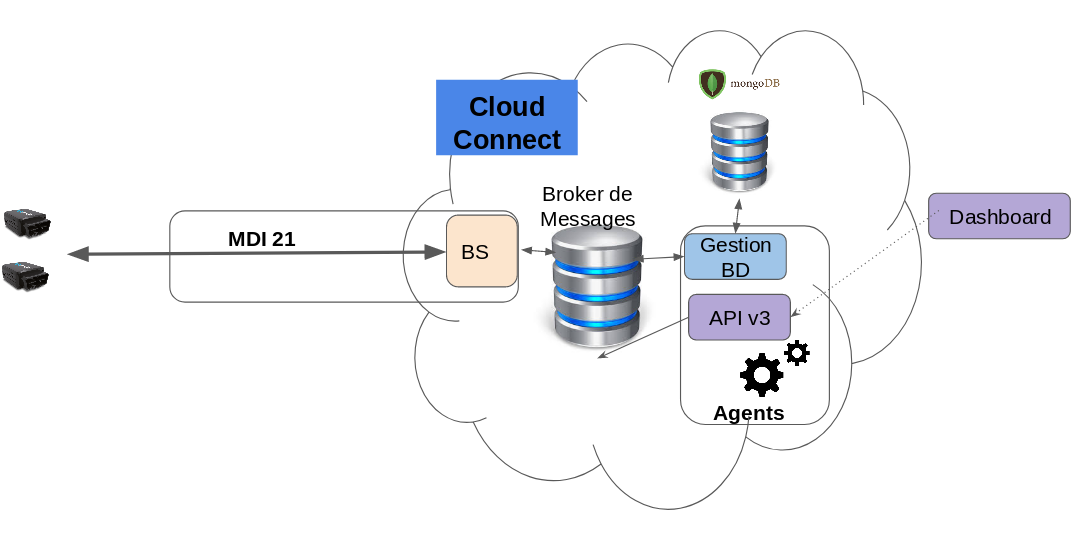
\includegraphics[scale=0.4]{\images/cc.png}
            \caption{L'architecture de CloudConnect}
        \end{figure}

        \gls{CC} comporte plusieurs composants : 
        \begin{itemize}
            \renewcommand{\labelitemi}{$\bullet$}
            \item  un \gls{BS} qui est le composant d'échange de messages entre le cloud et 
            les OBD. Il consiste le point d'entrée du cloud.
            \item  un broker de message pour les systèmes Big Data
            \item  un ensemble de services qui sont accéder à partir de APIV3 
            \item une base de données pour le stockage des données 
            \item un dashboard pour l affichage des données et l acces visuel 
            des services au clients 
        \end{itemize}
        \vspace{0.2cm}

        \gls{mdi21} est le protocole  ASN1 fait maison, conçu pour la communication entre boîtiers et Cloud.
        //développé un peu sur MD21

       
    \break

    \subsection{De \gls{CC} à \gls{CN}}
        Exprimer le besoin du changement d'architecture. 
        Autour de .. 
        Développement des agents : Un Framework interne est utilisé pour simplifier le développement des différents 
        agents en langage ruby. Ce framework fournit un ensemble de fonctions qui permettent, entre autres, d’accéder au 
        courtier de messages en lecture et en écriture. Concernant les agents à état, le framework ne fournit pas 
        de mécanismes pour simplifier la gestion de leurs états. La gestion de l’état est donc laissée aux développeurs.\\[0.3cm]
        Déploiement des agents : les agents sont exécutés de manière parallèle. En d’autres termes, un agent peut avoir 
        plusieurs instances déployées dans différentes machines. Les différentes instances d’un même agent partagent 
        le traitement du flux des événements mais ne communiquent pas entre eux. Le déploiement ainsi que la maintenance 
        d’un agent se traduisent par une mise-à-jour des fichiers de configuration des machines exécutant l’agent via le logiciel Chef.\\ [0.3cm]

        Solution :  Création d‘un autre Cloud afin de revoir l’architecture logicielle et technique de Cloud 
        Connect afin de simplifier le développement des agents, leurs déploiements ainsi que leurs maintenances et 
        de permettre à des développeurs externes de l’entreprise de coder leurs propres agents.



        \begin{figure}[ht]
            \centering
            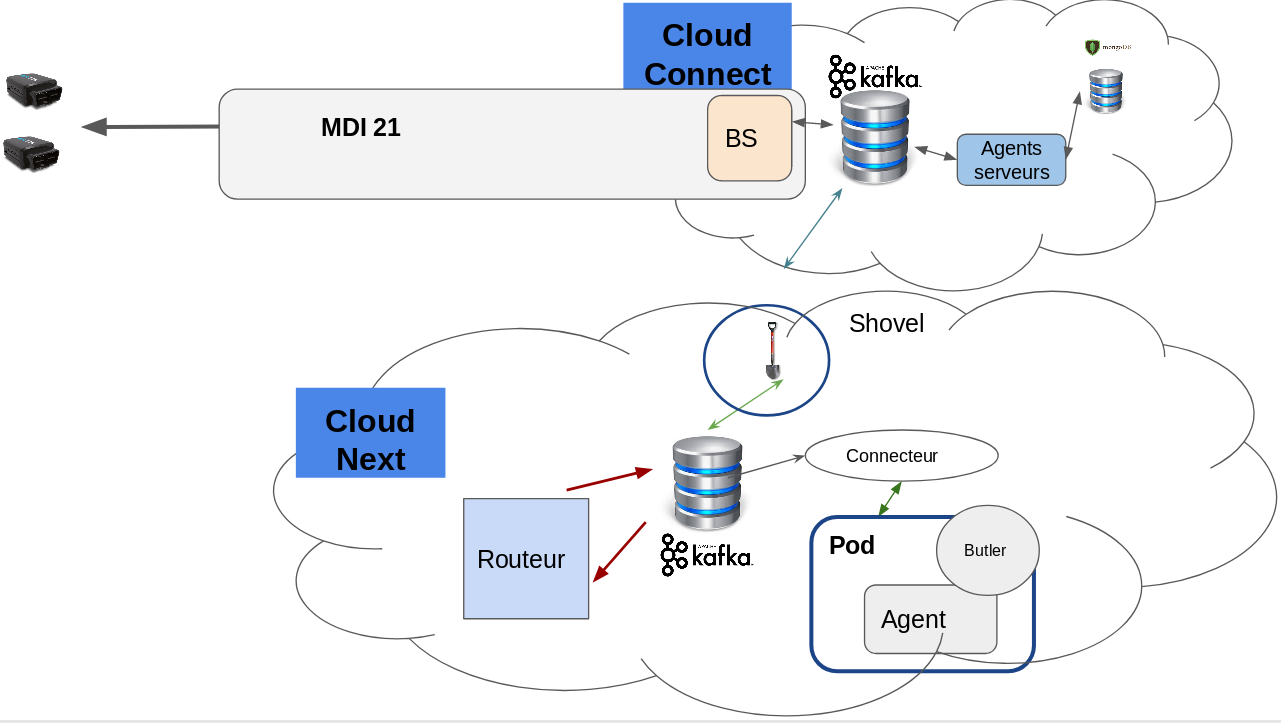
\includegraphics[scale=0.4]{\images/cn.png}
            \caption{L'architecture du cloud avec CloudNext}
        \end{figure}

        \vspace{0.2cm}

       

       

        \subsection{Données du cloud }

        Format : 

        Track : 
        Message : 
        


        Paragraphe sur le language Go : 
        Go est un jeune language de programmation système
        fascinant. Ce language compilé hérite des idées des paradigmes de
        programmation impérative et fonctionnelle. Il définit des concepts et
        des règles qui assurent à l'utilisateur des binaires .\\[0.3cm]
       
      
        Le but de cette explication est de montrer la différence considérable
        avec d'autres langages de programmation. Un lecteur intéressé pourra
        apprendre le langage pour plus d'informations.

        MD30, Un nouveau protocol de communication dongle-cloud